% TikZ 复刻。原图：assets/min-deviation-setup.png
% 回退：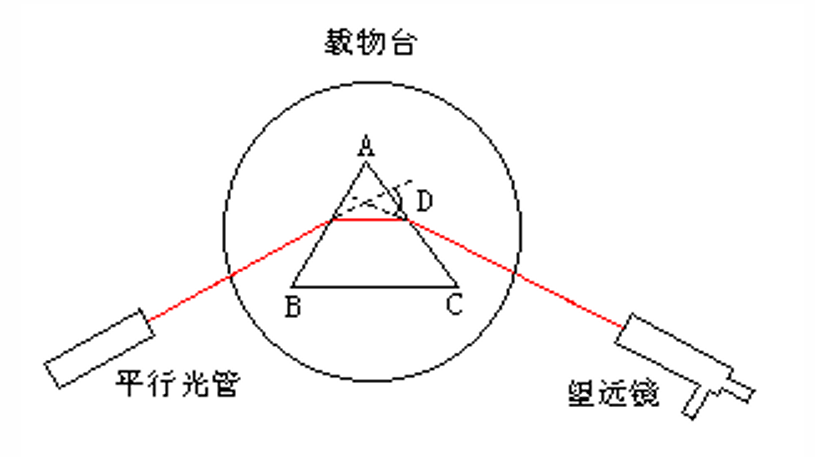
\includegraphics[width=\linewidth]{assets/min-deviation-setup.png}
\begin{tikzpicture}[>=Stealth, font=\small]
  % stage
  \draw[thick] (0,0) circle (1.15);
  % prism, apex up-right for min-deviation geometry
  \coordinate (A) at (0.15,0.62);
  \coordinate (B) at (-0.72,-0.42);
  \coordinate (C) at (0.78,-0.28);
  \draw[thick, fill=gray!12] (A)--(B)--(C)--cycle;
  \node[font=\scriptsize] at (0.05,0.05) {棱镜};
  % collimator on the left
  \draw[thick] (-3.55,-0.28) rectangle (-1.55,0.28);
  \draw[thick] (-1.55,-0.16) -- (-1.20,-0.16) -- (-1.20,0.16) -- (-1.55,0.16);
  \node[below] at (-2.55,-0.28) {平行光管};
  % telescope at deviation angle, lower right
  \begin{scope}[rotate around={-38:(1.85,-1.15)}]
    \draw[thick] (1.35,-1.38) rectangle (3.35,-0.82);
    \draw[thick] (1.35,-1.26) -- (1.05,-1.26) -- (1.05,-0.94) -- (1.35,-0.94);
  \end{scope}
  \node at (2.85,-1.85) {望远镜};
  % rays
  \draw[->, thick] (-1.18,0) -- (-0.55,-0.12);
  \draw[thick] (-0.55,-0.12) -- (0.35,-0.05);
  \draw[->, thick] (0.55,-0.18) -- (1.15,-0.72);
  \node[above] at (-2.55,0.28) {入射光};
  \node[right] at (1.20,-0.55) {出射光};
\end{tikzpicture}
